\chapter{GIMME Communication Protocol}
The GIMME Communication Protocol (GCP) is meant to be used with the GIMME system currently being developed at Mälardalens Högskola. GCP can communicate through raw Ethernet or USB and is primarily designed to transfer raw image data and Harris data but it also supports other custom data types in matrix or array form. GCP is designed as a layered header model, where a frame header is actually multiple headers layered on each other. Fault tolerance is not a priority in GCP because it is intended for use with streaming data, as a result there is no error correction if a frame is corrupt with the exception of certain control frames that require an acknowledgment to be sent as a reply.
\section{Requirements}
The GIMME system supports raw Ethernet and USB communication, GCP should be able to use both medias to transmit data.
\\
The data that is transmitted is real-time streaming data which favors a high throughput over error correction. If some frames are lost or corrupt it is not important to re-transmit them as it will not influence the overall result to a great extent.
\\
Although error correction is less important, the order of the data is important because it is mainly sequential image data that is transferred. If a frame is lost or corrupt it should be ignored and that data region should be skipped to prevent distorting the remainder of the image. For example, consider an image measuring 20x20 pixels and that each Ethernet frame could transfer 10 pixels. If one frame is lost (illustrated by the red rectangle in Figure \ref{fig:CameraLost}) the image would be distorted like the left image in Figure \ref{fig:CameraNotSeq} if the protocol ignored the lost frame completely. This result is unacceptable and can be solved by bypassing the missing pixels, thus continuing to reconstruct the image from the correct coordinates in the image, as can be seen in the right image in Figure \ref{fig:CameraSeq}.

\begin{figure}
\centering
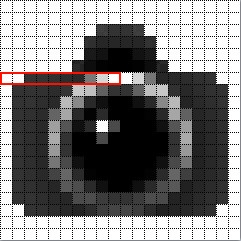
\includegraphics[width=0.4\textwidth]{CameraLost.jpg}
\caption{Original image to transmit}
\label{fig:CameraLost}
\end{figure}
\begin{figure}
\centering
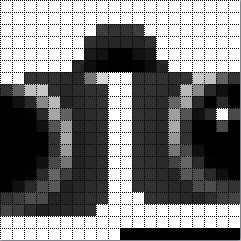
\includegraphics[width=0.4\textwidth]{CameraNotSeq.jpg}
\caption{If missing data after a lost frame is not skipped the resulting image look distorted}
\label{fig:CameraNotSeq}
\end{figure}
\begin{figure}
\centering
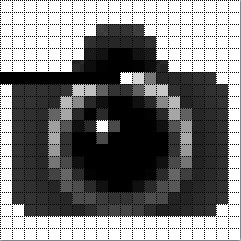
\includegraphics[width=0.4\textwidth]{CameraSeq.jpg}
\caption{Skipping over lost data by filling it with a solid color gives a more correct result}
\label{fig:CameraSeq}
\end{figure}

Protocol headers should be expandable and have room for future extensions. The headers follow a layered model, where the headers are put on top of each other. This provides an easy way to extend the protocol with other types of headers in the future and allows for more flexibility when attempting to minimize the headers to provide further throughput. GCP will use one mandatory header and a series of supplementary headers that describes the actual contents of a transaction. The supplementary headers will only appear in the first frame of a transaction, the subsequent frames will omit the header to further optimize throughput. If the frame containing the supplementary header is lost, the subsequent frames will be discarded since the contents of the transaction is unknown.
\\
Configuring compatible devices as well as being able to read and write the memory of these devices. The configuration options can vary between different devices and therefore needs to be as general as possible.
\\
In addition to simple polling for data there is support for subscription based transactions where it is possible to subscribe to specific types of data from individual devices on the network is.
\\
Compatible devices on the network should be automatically detected and identified through a handshake containing information that describes the features of the device.

\subsection{GCP Functionality}
GCP allows the following functionality based on the requirements,
\begin{itemize}
\item Transferring data through
	\begin{itemize}
	\item Raw Ethernet
	\item USB
	\end{itemize}
\item Transfer various types of predefined and general data
	\begin{itemize}
	\item Image data
	\item Harris algorithm data
	\item General arrays
	\item General matrices
	\end{itemize}
\item Dynamic headers
	\begin{itemize}
	\item Layered headers
	\item Minimizing use of headers to increase throughput
	\end{itemize}
\item Subscription based on
	\begin{itemize}
	\item Device ID
	\item Data type
	\end{itemize}
\item Automatic handshaking that
	\begin{itemize}
	\item Identifies a GCP compatible device
	\item Creates a handle to the device
	\item Get information about supported data modes and protocol versions
	\end{itemize}
\item Ping devices to verify they are still on the network
	\begin{itemize}
	\item Broadcast
	\item Single target
	\end{itemize}
\item Device configuration over the network
\item Read on-board memory
\item Write on-board memory
\end{itemize}

\subsection{PC requirements}
GCP needs to work on both Windows and Linux since both operating systems are used in conjunction with the GIMME device. This requires a driver that handles the communication layer and a API that enables developers to communicate through GCP. The driver will assemble and disassemble data into frames forming transactions. Transactions that are in the process of being received will be put in a temporary buffer until the transaction is completed, after completion the data will be moved to a buffer, either waiting for the user to fetch it or being dispatched to a callback function.
\\
OpenCVAda will be used to process image and data received from the network so an interface between GCP and OpenCVAda is beneficial to make development easier. This will add support to convert transactions to appropriate OpenCVAda types such as Ipl_Image and Cv_Mat.
\\
Since GCP supports subscription based transactions the driver should provide callback functions to automatically handle incoming subscribed transactions. When a new transaction is received it will be compared against the subscription list, if the device is subscribed and contains the desired data the transaction will be dispatched to a callback associated with the subscription.

\section{Design}
\subsection{Header structure}
Each transaction sent from a camera device is sent as a series of raw Ethernet frames (or equal ones over USB) with a constant header. The first frame in each transaction will have a specification header that details what type of transaction is sent, the specification header is different for all types of transactions. The last frame in a transaction will have an EOF flag set to signal that the transaction is terminated.

\begin{figure}
\centering
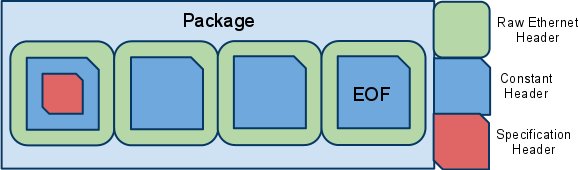
\includegraphics[width=1.0\textwidth]{Transaction.png}
\caption{Representation of a transaction (series of raw Ethernet frames)}
\label{fig:Transaction}
\end{figure}

\subsection{Raw Ethernet header}
\begin{figure}
\centering
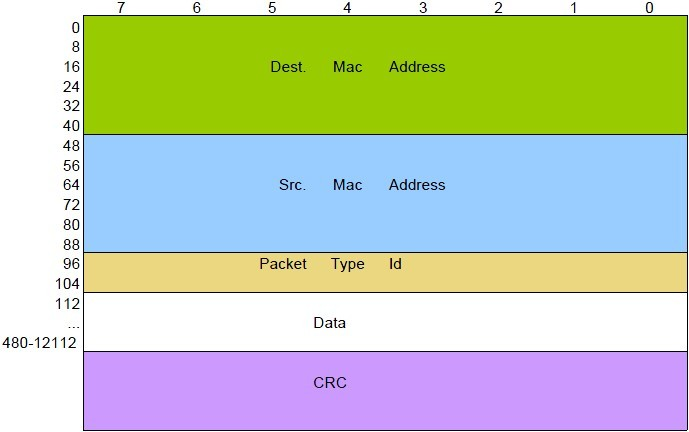
\includegraphics[width=1.0\textwidth]{RawEthernetHeader.jpg}
\caption{Raw Ethernet header}
\label{fig:RawEthernetHeader}
\end{figure}

\begin{description}
\item [Bit 0:47 - Dest. Mac Address] The address to the intended recipient of the Ethernet frame. The mac address FF-FF-FF-FF-FF-FF is used to broadcast messages to all devices on the network.
\item [Bit 48:95 - Src. Mac Address] The senders address.
\item [Bit 96:111 - Packet Type Id] Describes which type of Ethernet protocol is used, for this protocol only the IEEE802.3 Length Field is viable which range from 0x0000-0x05DC (0-1500).
\item [Bit 112:479-12111 - Data] This field contains the payload of the Ethernet frame, it can range from 48-1500 byte.
\item [Bit 480:501-12112:12143 - CRC] The end of the frame is a cyclic redundancy check to verify that the message has not been corrupted.
\end{description}
\subsection{Constant and specification headers}
All Ethernet frames sent will use the constant header in addition to the raw Ethernet header, the first Ethernet frame in each transaction will be a specification header for the different types of transactions.
\subsubsection{Constant header}
\begin{figure}
\centering
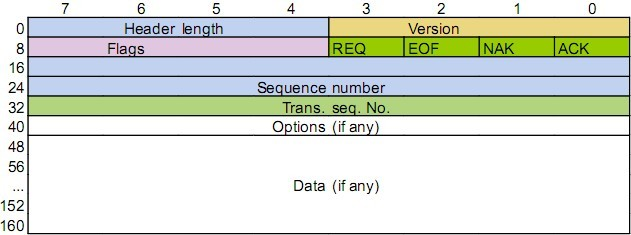
\includegraphics[width=1.0\textwidth]{MainHeader.jpg}
\caption{Mandatory protocol header}
\label{fig:MainHeader}
\end{figure}
\begin{description}
\item [Bit 0:3 - Version] Version of the protocol being used.
\item [Bit 4:7 - Header Length] If the header contains extra data (i.e. handshake) this field  specifies how many extra bytes of data the header contains. See Bit 40:159 - Data for further information.
\item [Bit 8 - ACK] This bit signifies that the transaction is a response to a request.
\item [Bit 9 - NAK] If a corrupt or erroneous frame is received, a mirrored frame with this bit set will be transmitted back to the sender.
\item [Bit 10 - EOF] The last frame of each transaction will have this bit set to signify that the end of the transaction is reached.
\item [Bit 11 - REQ] This bit is used to make a request of some description (i.e. requesting image data).
\item [Bit 12:15 - Flags] The flags field is used for the remaining flags that are mutually exclusive.
	\begin{itemize}
	\item 0000: No flags
	\item 0001: Ping
	\item 0010: Configure
	\item 0011: Handshake
	\item 0100: Subscribe
	\item 0101: Data
	\item 0110: Memory
	\item 1111: Extended flags
	\end{itemize}
\item [Bit 16:31 - Seq. No.] A sequence number that describes which frame within a transaction this is. The sequence number is reset for each transaction of frames.
\item [Bit 32:39 - Trans. seq. No.] If a device is transmitting multiple transactions with separate data of the same type in parallel it is necessary to be able to differentiate between them. The transaction sequence number is used to separate transactions from each other. When a transaction is transmitted it will keep the same transaction sequence number throughout the transmission of the transaction, the sequence number will however be incremented for each frame within the transaction.
\item [Bit 40:47 - Options] This field is not part of the standard header. If Extended flags is set this field will give access to one additional byte of customizable flags that can be application specific.
\item [Bit 48:167 - Data] This field is not part of the standard header. Some header flags require additional data (i.e. handshake), this field is used in those cases to store the extra data associated with such flags. The Header Length field specifies the size of this field in whole bytes, if a whole byte is not used the remaining bits shall be padded with zeros’.
The bit offset for this can be either 32 or 40 if Extended flags is false or true respectively.
\end{description}
\subsubsection*{Handshake}
When a device becomes available on the network it is necessary to determine if it is a compatible device and also what features are available on the device. The handshake is performed with a 1 byte mask followed by information about the device. The mask is used as an identifier which together with the rest of the header make up a unique message to identify compliant devices. The reply from any compatible device will be mirrored from the handshake request up to the 32nd bit with the exception of having the ACK flag set in the reply. After the 32nd bit follows the information about the device such as device type and available data structures that can be used when communicating with it.

\begin{figure}
\centering
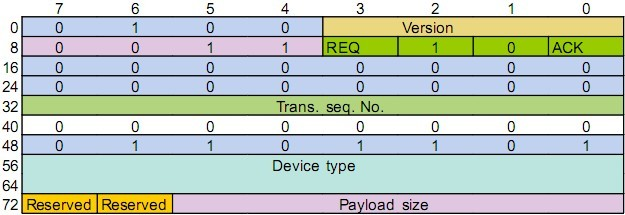
\includegraphics[width=1.0\textwidth]{HandshakeHeader.jpg}
\caption{Handshake header}
\label{fig:HandshakeHeader}
\end{figure}

\begin{description}
\item [Bit 0:3 - Version] Version of the protocol being used.
\item [Bit 4:7 - Header Size] Always 0100 since there is 4 extra bytes in the handshake header.
\item [Bit 16:31 - Seq. No.] Always 0 not used.
\item [Bit 32:39 - Hndshake mask] This field contains a mask that is used to confirm that the handshaking device is compatible. The fields value is constant and should be set to 0x6D.
\item [Bit 40:55 - Device type] This field describes what type of device the sender is.
\item [Bit 56:61 - Payload size] Amount of bytes added as payload, used to describe the functionalities available. 
\item [Bit 62:63 - Reserved] Reserved for future use.
\end{description}

\subsubsection*{Ping}
Message used to check for devices currently on the network. This can be used with a broadcast address to check all devices on the network at once.
\begin{figure}
\centering
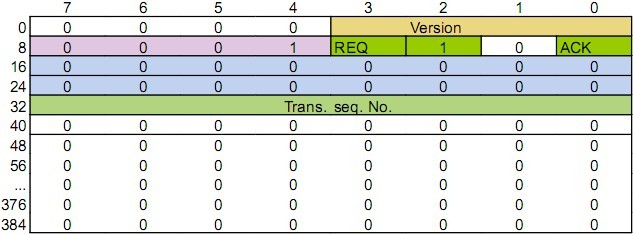
\includegraphics[width=1.0\textwidth]{PingHeader.jpg}
\caption{Ping header}
\label{fig:PingHeader}
\end{figure}

\begin{description}
\item [Bit 0:3 - Version] Version of the protocol being used.
\item [Bit 8 - ACK] Acknowledges a request.
\item [Bit 10 - EOF] Always 1 since a ping can only be one frame long.
\item [Bit 11 - REQ] Requests a response from the destination.
\item [Bit 12:15 - Flags] Always 0001 which is the flag for ping.
\end{description}
\subsubsection*{Subscription}
\begin{figure}
\centering
\includegraphics[width=1.0\textwidth]{SubscriptionHeader.jpg}
\caption{Subscription header}
\label{fig:SubscriptionHeader}
\end{figure}
\begin{description}
\item [Bit 0:3 - Version] Version of the protocol being used.
\item [Bit 4:7 - Header length] Set to 0011 to denote that the frame header is two bytes longer then the normal constant header.
\item [Bit 8 - ACK] Set when acknowledging a new subscription.
\item [Bit 9 - NAK] Set when not acknowledging a new subscription.
\item [Bit 10 - EOF] Always set to 1 since a subscription transaction is only one frame.
\item [Bit 11 - REQ] Set when requesting that a new subscription should be started.
\item [Bit 12:15 - Flags] Always 0100 which is the flag for subscription.
\item [Bit 16:31 - Seq number] Always 0.
\item [Bit 32 - Any] Subscribe to any data sent from the device. (Byte 6 and 7 is ignored.)
\item [Bit 33 - Time] If set to 1 requested data will be sent at the chosen interval. (Byte 7)
\item [Bit 34:39 - Reserved] Reserved bits for future use.
\item [Bit 40:45 - Data mode] See Image and data headers for the possible data modes that can be subscribed to.
\item [Bit 46:47 - Data version] See above.
\item [Bit 48:55 - Ms Delay] The delay between the transaction sent, in milliseconds. (I.E. how many “image frames” per second that is sent.)
\item [Bit 56 - Reserved] Reserved bit for future use.
\end{description}

\subsubsection{Specification headers}
The specification headers are used at the start of each transaction to specify the type of transaction and what it contains due to the dynamic headers requirement, this header will only be used on the necessary frames and the constant and Ethernet headers will be used on every Ethernet frame including the one with the specification header.
\subsubsection*{Image and data headers}
Except for an image the data headers can reference with two types of data templates array and matrix. There is also room for around 60 specific data types like Harris data. The 2 bit version flag is for when the device supports more then one version of a single header or to indicate a rewrite between versions of the device. 

\begin{figure}
\centering
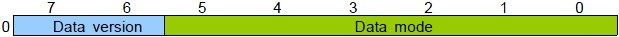
\includegraphics[width=1.0\textwidth]{DataTypeHeader.jpg}
\caption{Data type header}
\label{fig:DataTypeHeader}
\end{figure}

\begin{description}
\item [Bit 0:5 - Data Mode] Data modes available:
	\begin{itemize}
	\item 000000 - Image
	\item 000001:011111	- Matrices
	\item 100000 -  Harris
	\item 100001:111111 - Arrays
	\end{itemize}
\item [Bit 6:7 - Data Version] Version explanation:
	\begin{itemize}
	\item 00 - Current version
	\item 01 - Extra version 1
	\item 10 - Extra version 2
	\item 11 - Deprecated version
	\end{itemize}
\end{description}
While the matrix and array headers might not be able to do a full specification that can be used to create a type without more knowledge on the PC side, the headers should be able to represent any realistic type needed. Using the array or the matrix header without creating a new definition on both sides should not be done, since it will not be possible to distinguish between different implementations of the templates. 
\subsubsection*{Image header}
\begin{figure}
\centering
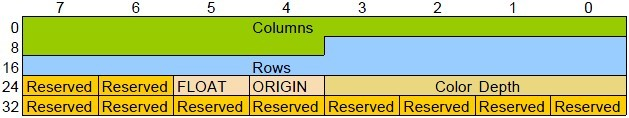
\includegraphics[width=1.0\textwidth]{ImageHeader.jpg}
\caption{Image data header}
\label{fig:ImageHeader}
\end{figure}

\begin{description}
\item [Bit 0:11 - Columns] Columns in the image, between 1 and 4096.
\item [Bit 12:23 - Rows] Rows in the image, between 1 and 4096.
\item [Bit 24:27 - Color Depth] Color depths available:
	\begin{itemize}
	\item 0000 - 1 bit
	\item 0001 - 8 bit gray (8)
	\item 0010 - 8 bit color(3,3,2)
	\item 0011 - 15 bit (5,5,5)
	\item 0100 - 24 bit (8,8,8)
	\item 0101 - 30 bit (10,10,10)
	\item 0110 - 36 bit (12,12,12) (GIMME camera standard)
	\item 0111 - 48 bit (16,16,16)
	\item 1000:1111 - Reserved for future colors
	\end{itemize}
\item [Bit 28 - ORIGIN] Top left origin (1) or Bottom left origin (0).
\item [Bit 29 - FLOAT] Color is represented as 0.0 to 1.0 instead of an integer value.
\item [Bit 30:39 - Reserved] Reserved bits for future use.
\end{description}

\subsubsection*{Matrix header}
A matrix behaves like a image except that it allows for anonymous types as elements instead of a color. Each element have a maximum size of 8191 bytes with a possible padding of 7 bits. 

\begin{figure}
\centering
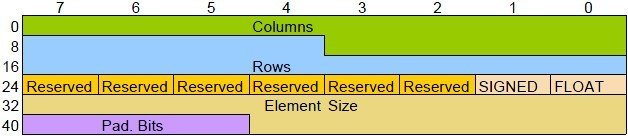
\includegraphics[width=1.0\textwidth]{MatrixHeader.jpg}
\caption{Matrix data header}
\label{fig:MatrixHeader}
\end{figure}

\begin{description}
\item [Bit 0:11 - Columns] Columns in the matrix, between 1 and 4096.
\item [Bit 12:23 - Rows] Rows in the matrix, between 1 and 4096.
\item [Bit 24 - FLOAT] Elements are float values instead of integer values.
\item [Bit 25 - SIGNED] Elements are signed or unsigned.
\item [Bit 26:31 - Reserved] Reserved bits for future use.
\item [Bit 32:44 - Element Size] Total size of the element in the matrix.
\item [Bit 45:47 - Padding Bits] Used if element size is not a even byte.
\end{description}

\subsubsection*{Array header}
The array type has a maximum length of roughly 16.8 million elements where each element has a combined maximum size of 8191 bytes with a padding of 7 bit possible. 
\begin{figure}
\centering
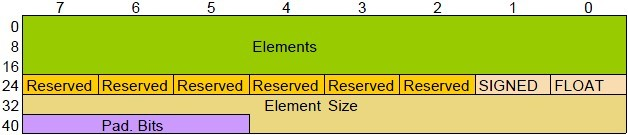
\includegraphics[width=1.0\textwidth]{ArrayHeader.jpg}
\caption{Array data header}
\label{fig:ArrayHeader}
\end{figure}

\begin{description}
\item [Bit 0:23 - Elements] Number of elements in the array.
\item [Bit 24 - FLOAT] Elements are float values instead of integer values.
\item [Bit 25 - SIGNED] Elements are signed or unsigned.
\item [Bit 26:31 - Reserved] Reserved bits for future use.
\item [Bit 32:44 - Element Size] Total size of the element in the array.
\item [Bit 45:47 - Padding Bits] Used if element size is not a even byte.
\end{description}
\subsubsection*{Harris data header}
Will be a array header with only elements as the parameter allowed to be changed.
\subsubsection*{Configuration header}
Configuration of a device on the network can be done with the configuration header. The header contains the number of registers to configure, the size of the registers and the size of the registers addresses.
\\
The header is followed by a payload consisting of pairs of addresses and values. The EOF flag will be set in the last frame denoting the end of the configuration transaction.
\\
Each frame will be acknowledged by the receiver with a ACK-frame, a corrupt message will trigger a NAK-frame to be sent. If a frame is lost or corrupt the transmitter will re-transmit the frame upon receiving the NAK-frame or after failing to receive a response within a certain delay.

\begin{figure}
\centering
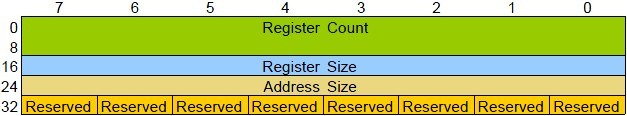
\includegraphics[width=1.0\textwidth]{ConfigurationHeader.jpg}
\caption{Configuration header}
\label{fig:ConfigurationHeader}
\end{figure}

\begin{description}
\item [Bit 0:15 - Register Count] Number of registers that will be configured.
\item [Bit 16:23 - Register Size] The size of the registers in bytes.
\item [Bit 24:31 - Address Size] The address size in bytes.
\item [Bit 32:39 - Reserved] Reserved bits for future use.
\end{description}

\subsubsection*{Memory header}

Send or receive memory from start address to end address.

\begin{figure}
\centering
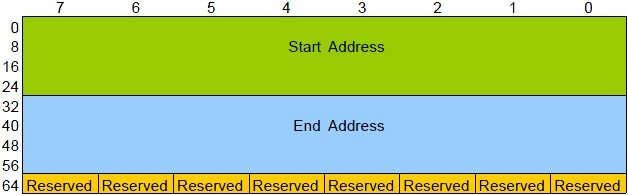
\includegraphics[width=1.0\textwidth]{MemoryHeader.jpg}
\caption{Memory header}
\label{fig:MemoryHeader}
\end{figure}

\begin{description}
\item [Bit 0:31 - Start Address] The beginning of the memory space where data will be read/written.
\item [Bit 32:63 - End Address] The end of the memory space where data will be read/written.
\item [Bit 64:71 - Reserved] Reserved bits for future use.
\end{description}

\subsection{PC GCP driver design}

\subsubsection{System design}

The driver on the PC side will be driven by different threads that takes care of the communication between a user API and the network. Data will be received according to these steps:

\begin{enumerate}
\item Frames from the network are sorted into their appropriate frame buffer.
\item A thread responsible for the frame buffer will start assembling the frames into a complete transaction.
\item When the transaction is finished, the transaction is put into a transaction buffer.
\item The API fetches the transaction on a users request, or dispatches it to an appropriate callback.
\end{enumerate}

When transmitting data the steps are done in reverse

\begin{enumerate}
\item The API creates a transaction from data provided by the user.
\item The transaction is put into an outgoing transaction buffer.
\item A thread managing the outgoing communication disassembles a transaction into frames.
\item The frames are put into a frame buffer waiting to be sent out on the network.
\end{enumerate}

A simplified view of the communication interface (see figure \ref{fig:GcpPc}) could be described as different layers. There is a network layer which is the physical medium actually transporting the data between endpoints. A frame buffer layer hold incoming and outgoing frames waiting to be transmitted or processed. After the frame buffer layer is a layer of threads that assemble and disassemble data from the buffer layers. The threads are followed by layer of transaction buffers that contain complete data either waiting to be fetched by the API or to be disassembled and transmitted out on the network. The last layer is the API layer which is used by developers to send and receive data from the network.

\begin{figure}
\centering
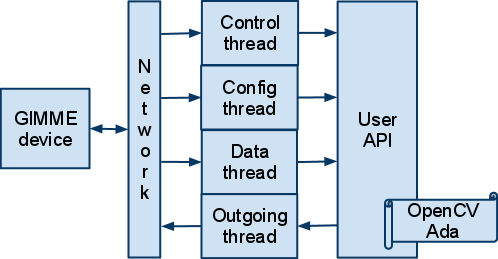
\includegraphics[width=1.0\textwidth]{GcpPc.png}
\caption{Communication protocol design}
\label{fig:GcpPc}
\end{figure}

\subsubsection{Network layer}
Handles sending and receiving of raw Ethernet frames. Frames received will be sent to the appropriate frame buffer, while frames that are sent is taken from the outgoing frame buffer.
\subsubsection{Frame buffer layer}
The buffers in this layer contain frames received from the network or waiting to be transmitted out on the network. Each connected device has its own set of buffers that are associated with it. In the case of a buffer overflow the oldest frames will be dropped since new data is preferred over old data with the exception that a transactions first frame will always have a higher priority since it contains vital information about the transaction. If that frame is dropped the remaining frames of that transaction are useless.
\subsubsection{Thread layer}
This layer consists of a number of threads, each responsible for a frame buffer and a transaction buffer (see figure \ref{fig:GcpThread}). The threads handling incoming frames read a frame from the frame buffer and extracts the data into the appropriate place in a transaction buffer. There is one thread that handles outgoing data, the thread works the opposite way from the incoming threads. It reads data from the transaction buffer and disassembles it into frame that are put into the frame buffer waiting to be transmitted.

\begin{figure}
\centering
%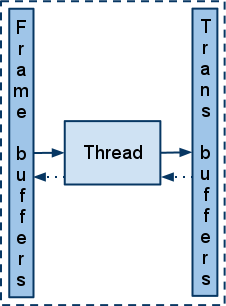
\includegraphics[width=1.0\textwidth]{GcpThread.png}
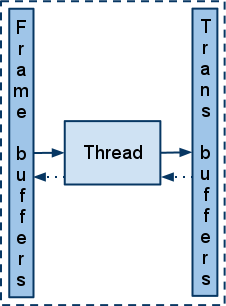
\includegraphics[scale=0.7]{GcpThread.png}
\caption{Thread layer layout}
\label{fig:GcpThread}
\end{figure}
\subsubsection{Transaction buffer layer}
This layer contains buffers where complete transactions are stored. Transactions that have been received from the network are assembled and put in the appropriate buffer ready to be fetched by the user. Each connected device has its own set of buffers that are associated with it. These buffers can only contain one transaction since it is only the latest data that is relevant, so if a new transaction is completed before the current one has been fetched it will be overwritten by the new transaction.
\subsubsection{API layer}
The API contains functions to enable developers to interact with the network. It stores information about available devices and maintains handles to interact with those devices. The API provides functions to create GCP headers and transactions as well as functions that transmit and receive data from the network. Some of the native OpenCVAda types are supported directly in the API to make the transition from a GIMME device to OpenCVAda easier.